% !TEX encoding = UTF-8 Unicode

\documentclass[12pt]{report}
\usepackage[a4paper]{geometry}
\usepackage[myheadings]{fullpage}
\usepackage{fancyhdr}
\usepackage{lastpage}
\usepackage{graphicx, wrapfig, subcaption, setspace, booktabs}
\usepackage[english]{babel}
\usepackage{color}
\usepackage{hyperref}
\usepackage{array}
\usepackage{supertabular}
\usepackage{hhline}
\usepackage{enumitem}
\usepackage[T1]{fontenc}
\usepackage[utf8]{inputenc}
\usepackage{graphicx}

\newcommand{\HRule}[1]{\rule{\linewidth}{#1}}
\renewcommand{\theenumii}{\arabic{enumii}.}
\addto\captionsenglish{
	\renewcommand{\contentsname}{Innhold}
}
\onehalfspacing
\setcounter{tocdepth}{5}
\setcounter{secnumdepth}{5}
%-------------------------------------------------------------------------------
% HEADER & FOOTER
%-------------------------------------------------------------------------------
\pagestyle{fancy}
\fancyhf{}
\setlength\headheight{15pt}
\fancyhead[L]{Team D} 
\fancyhead[R]{Universitetet i Bergen}
\fancyfoot[R]{Page \thepage\ of \pageref{LastPage}}
%-------------------------------------------------------------------------------
% TITLE PAGE
%-------------------------------------------------------------------------------
\begin{document}
\title{ \normalsize \textsc{}
		\\ [2.0cm]
		\HRule{0.5pt} \\
		\LARGE \textbf{\uppercase{Bilspill}}
		\HRule{2pt} \\ [0.5cm]
		\normalsize \today \vspace*{5\baselineskip}}
\date{}
\author{
		Team D  \\ 
		Universitetet i Bergen \\
		Informatikk }
\maketitle
\tableofcontents
\newpage
%-------------------------------------------------------------------------------
% BODY
%-------------------------------------------------------------------------------
\section*{Bruksm{\o}nstertekst:}
\addcontentsline{toc}{section}{Bruksm{\o}nstertekst:}

\textbf{Tittel}: F{\aa} h{\o}yest mulig score
\bigskip \\
\textbf{Akt{\o}rer}: Spiller, System
\bigskip \\
\textbf{Prim{\ae}rakt{\o}r}: Spiller
\bigskip \\
\textbf{Tid}: Varierende, avhengig av spillers prestasjon
\bigskip \\
\textbf{M{\aa}l}: F{\aa} h{\o}yest mulig highscore f{\o}r man g{\aa}r tom for bensin
\bigskip \\
\textbf{Pre-conditions:} Spillet er startet p{\aa} en datamaskin
\subsubsection*{Hovedflyt:}
\begin{enumerate}
\item Systemet viser startmeny
\item Spiller velger {\aa} starte spillet
\item Systemet startet spillet
\item Spiller styrer bil med venstre/h{\o}yre piltast
\item Systemet flytter bilen i takt med tastetrykk
\item Spiller unng{\aa}r hindre
\item Spiller kj{\o}rer p{\aa} folk
\item Systemet legger til én mynt i spillerens inventar for hver person som blir p{\aa}kj{\o}rt
\item Spiller kj{\o}rer over en bensintank
\item Systemet legger til bensinen i en "counter", som gj{\o}r at spilleren kan kj{\o}re lengre
\item Spiller g{\aa}r tom for bensin
\item Systemet stopper spillet
\item Systemet lagrer spillers score
\item Systemet viser spillers score og highscore
\item Systemet viser startmeny
\end{enumerate}
\pagebreak
\subsubsection*{Alternative handlinger:}
\begin{enumerate}[label=\Alph*]
\item 
\bigskip
\begin{enumerate}
\item @1 Spiller klikker p{\aa} oppgradering
\item Systemet viser spiller mulige oppgraderinger 
\item Spiller kj{\o}per oppgradering
\item Systemet oppgraderer bilen
\item Spiller klikker seg tilbake til startmenyen
\item Gjenoppta @1
\end{enumerate}
\item 
\bigskip
\begin{enumerate}
\item @1 Spiller trykker p{\aa} innstillingsknapp
\item Systemet viser spiller mulige innstillinger for spillet
\item Spiller endrer innstillinger
\item Systemet lagrer instillingene
\item Gjenoppta @1
\end{enumerate}
\item
\bigskip
\begin{enumerate}
\item @3, 4, 5 Spiller pauser spiller
\item Systemet viser en pauseskjerm
\item Spiller velger {\aa} avslutte spillet
\item Gjenoppta @13
\end{enumerate}
\item
\bigskip
\begin{enumerate}
\item @3, 4, 5 Spiller pauser spiller
\item Systemet viser en pauseskjerm
\item Spiller velger {\aa} gjenoppta spillet
\item Gjennoppta @3
\end{enumerate}
\end{enumerate}
\pagebreak
\section*{Bruksm{\o}nsterdiagram:}
\addcontentsline{toc}{section}{Bruksm{\o}nsterdiagram:}
\vspace{4cm}
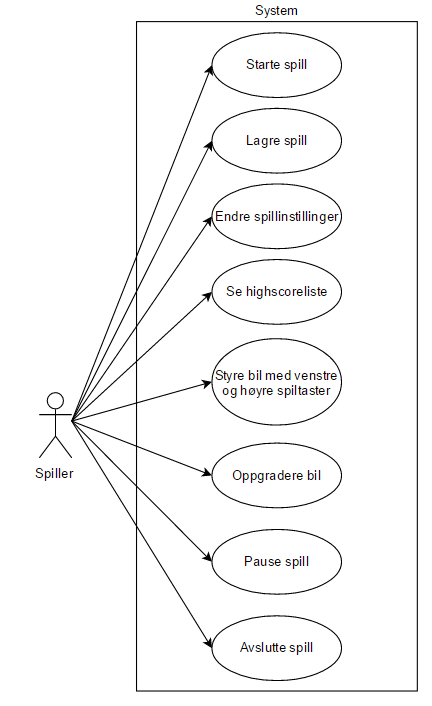
\includegraphics[width=0.8\textwidth,natwidth=500,natheight=642]{use_case_diagram_b.png}
\end{document}